% !TEX TS-program = xelatex
% !TEX encoding = UTF-8 Unicode

% Tennessee Technological University
% ENGR1120-021 - GSET - Summer 2021
% Tristan Hill - June 03, 2021
% Module 2 - Variables, Expressions, and Assignment
% Lecture 2 


\documentclass[fleqn]{beamer} % for presentation (has nav buttons at bottom)

\usepackage{/home/thill/Documents/lectures/cpp_workshop/modules/cpp_lectures}

\newcommand{\MNUM}{2\hspace{2mm}} % Module number
\newcommand{\TNUM}{---\hspace{2mm}} % Topic number - single topic for now
\newcommand{\moduletitle}{Variables and Assignment} % Titles and Stuff
%\newcommand{\topictitle}{---} 

\newcommand{\sectiontitleI}{Types of Numbers} % More Titles and Stuff
\newcommand{\sectiontitleII}{Variables and Type}
\newcommand{\sectiontitleIII}{Assignment and Memory}
\newcommand{\sectiontitleIV}{A {\it Riddle} }
\newcommand{\sectiontitleV}{A C++ Example }

\newcommand{\btVFill}{\vskip0pt plus 1filll}

\setbeamercolor{title in head/foot}{fg=TTUgold} % this needs work...

\title{GSET - Programming with Mr. Hill}
\author{Tristan Hill\vspc \hspc Tennessee Technological University \hspc}
\date{Summer 2021}

\begin{document}

\lstset{language=MATLAB,basicstyle=\ttfamily\small,showstringspaces=false}

\frame{\titlepage \center\begin{framed}\Large \textbf{Module \MNUM - \moduletitle}\end{framed} \vspace{5mm}}

% Section 0 - Outline
\frame{
	
	\large \textbf{Module \MNUM - \moduletitle} \vspace{3mm}\\
	
	\begin{itemize}
	
		\item \hyperlink{sectionI}{\sectiontitleI} \vspc % Section I
		\item \hyperlink{sectionII}{\sectiontitleII} \vspc % Section II
		\item \hyperlink{sectionIII}{\sectiontitleIII} \vspc %Section III
		\item \hyperlink{sectionIV}{\sectiontitleIV} \vspc %Section IV	
		\item \hyperlink{sectionV}{\sectiontitleV} \vspc %Section V
	
	\end{itemize}

}


% Section I
\section{\sectiontitleI}

	% Section I - Frame I
	\begin{frame}[label=sectionI] \small
		\frametitle{\sectiontitleI}
		
		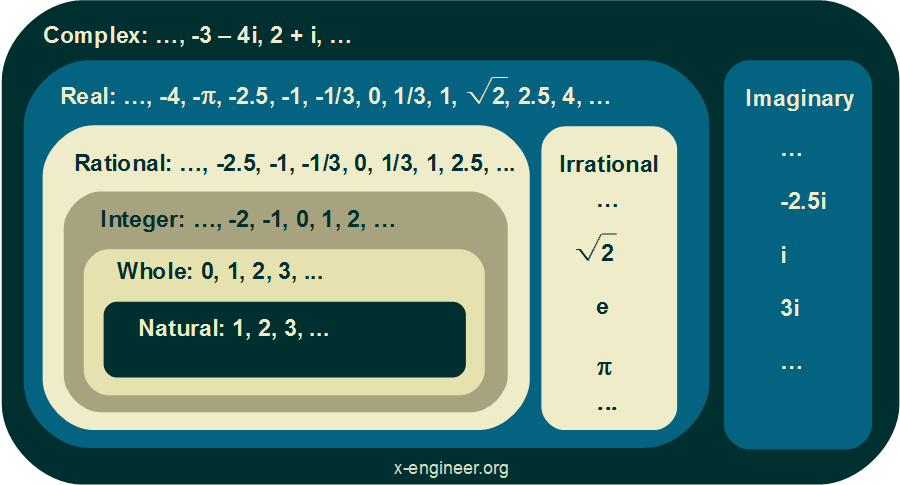
\includegraphics[scale=.35]{types_of_numbers.png} \\
		
				\tiny{Image: \href{https://x-engineer.org/undergraduate-engineering/mathematics/arithmetics/types-of-numbers/}{x-engineer.org}}
	
	\end{frame}

	%\section{\sectiontitleII}	
	
	% Section I - Frame II
	\begin{frame}[label=sectionI] \small
	\frametitle{\sectiontitleI}
	\bigskip
	
	\begin{multicols}{2}
		\begin{tabular}{|r|r|r|} \hline
			Binary 	& Decimal 	& Hexadecimal \\ \hline
			0		& 0			& 0 		\\ \hline	
			1		& 1			& 1 		\\ \hline
			10		& 2			& 2 		\\ \hline
			11		& 3			& 3 		\\ \hline
			100		& 4			& 4 		\\ \hline
			& 5			& 5 		\\ \hline
			& 6			& 6 		\\ \hline
			& 7			& 7 		\\ \hline
			& 8			& 8 		\\ \hline
			& 9			& 9 		\\ \hline
			& 10		& A 		\\ \hline
			& 11		& B 		\\ \hline
		\end{tabular}
		
		\begin{tabular}{|r|r|r|} \hline
			Binary 	& Decimal 	& Hexadecimal \\ \hline
			& 12		& C 		\\ \hline	
			& 13		& D 		\\ \hline
			& 14		& E 		\\ \hline
			& 15		& F 		\\ \hline
			& 16		&  		\\ \hline
			& 17		&  		\\ \hline
			& 18		&  		\\ \hline
			& 19		&  		\\ \hline
			& 20		&  		\\ \hline
			& 21		&  		\\ \hline
			& 22	    &  		\\ \hline
			& 23	    &  		\\ \hline
		\end{tabular}
	\end{multicols}
	
	\btVFill
	\tiny{some reference}		
	
\end{frame}

% Section I - Frame III
\begin{frame} \small
\frametitle{\sectiontitleI}
\bigskip

\begin{multicols}{2}
\begin{tabular}{|r|r|r|} \hline
	Binary 	& Decimal 	& Hex. \\ \hline
	0		& 0			& 0 		\\ \hline	
	1		& 1			& 1 		\\ \hline
	10		& 2			& 2 		\\ \hline
	11		& 3			& 3 		\\ \hline
	100		& 4			& 4 		\\ \hline
	& 			&  		\\ \hline
	& 			&  		\\ \hline
	& 			&  		\\ \hline
	& 			&  		\\ \hline
	& 			&  		\\ \hline
	& 		&  		\\ \hline
	& 		&  		\\ \hline
\end{tabular}

\begin{tabular}{|r|r|r|} \hline
	Binary\hspace{18mm} 	& Decimal 	& Hex. \\ \hline
	0		& 0			& 0 		\\ \hline	
	1		& 1			& 1 		\\ \hline
	10		& 2			& 2 		\\ \hline
	11		& 3			& 3 		\\ \hline
	100		& 4			& 4 		\\ \hline
	& 			&  		\\ \hline
	& 			&  		\\ \hline
	& 			&  		\\ \hline
	& 			&  		\\ \hline
	& 			&  		\\ \hline
	& 		&  		\\ \hline
	& 		&  		\\ \hline
\end{tabular}
\end{multicols}

\btVFill
\tiny{some reference}	
\end{frame}


% Section II
\section{\sectiontitleII}

	% Section II - Frame I
	\begin{frame}[label=sectionII,containsverbatim] \small
		\frametitle{\sectiontitleII}
	
	
			\begin{lstlisting}
			
				int val_A; 
				
				int val_B = 25;
			
			\end{lstlisting}
	
			A variable is a storage container.
			\begin{itemize}
				\item In C++ and many other programming languages, each variable has a type defined by the programmer. This is called {\BL Initialization}.
				\item In some programming languages, the type is hidden or abstracted away from the programmer. 
			\end{itemize}
	
		\end{frame}

	% Section II - Frame II
	\begin{frame} \small
		\frametitle{\sectiontitleII}
			
		Commonly Used Types in C++ and other languages \vspace{5mm}\\
		\renewcommand*{\arraystretch}{1.5}
		\begin{tabular}{|c|c|c|c|}\hline			
			Type & C++ Syntax & Purpose & Examples  \\ \hline
			Boolean & bool & state, logic & 1,0 (On,Off) \\ \hline 	
			Integer & int & arithmetic, counting & 1,2,56,-123 \\ \hline
			Floating Point & float & arithmetic, computation & 57,412.683 \\ \hline
			Double Float. & double & increased resolution & 124.000234567\\ \hline
			Character & char & human language & "Hello World"\\ \hline	 			
	
		\end{tabular}
	
	\btVFill
	{\tiny \href{https://www.tutorialspoint.com/cplusplus/cpp_data_types.htm}{Tutorials Point},\href{https://en.wikipedia.org/wiki/Single-precision_floating-point_format}{Wikipedia - Floating Point}}
	\end{frame}	

	% Section II - Frame III
	\begin{frame} \small
	\frametitle{\sectiontitleII}
	
	Variable type have limited range. \vspace{2mm}\\
	\renewcommand*{\arraystretch}{1.5}
	\begin{tabular}{|c|c|c|c|}\hline			
		Type & C++ Syntax & Min Value & Max Value  \\ \hline
		Boolean & bool &  0 (Off) & 1 (On) \\ \hline 	
		Unsigned Integer (4 bytes) & uint &  0 &  \\ \hline
		Signed Integer (4 bytes) & int &   &  \\ \hline
		Unsigned Short Int. (2 bytes) & uint &   &  \\ \hline
		Signed Short Int. (2 bytes) & int &   &  \\ \hline
		Floating Point (4 bytes) & float &  & \\ \hline
		Double Float. (8 Bytes) & double &  &\\ \hline
		Character & char &  &\\ \hline	 			
		
	\end{tabular}
	
	\btVFill
	{\tiny \href{https://www.tutorialspoint.com/cplusplus/cpp_data_types.htm}{Tutorials Point}}
\end{frame}


% Section III
\section{\sectiontitleIII}


	% Section III - Frame I
	\begin{frame}[label=sectionIII] \small
	\frametitle{\sectiontitleIII}
	
	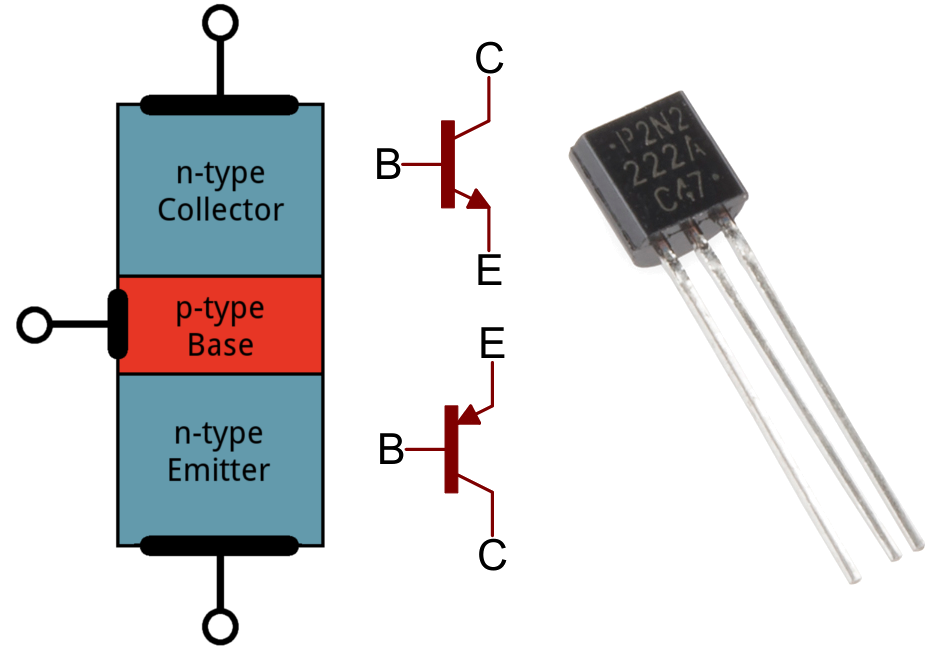
\includegraphics[scale=.15]{transistor_pnp}
	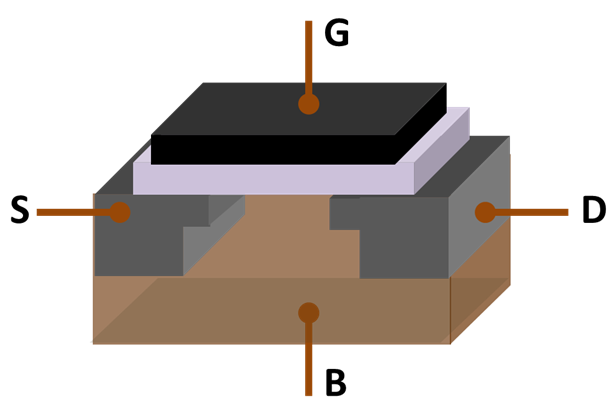
\includegraphics[scale=.25]{MOSFET_Structure.png}
	
	\btVFill
	\href{https://learn.sparkfun.com/tutorials/transistors/all}{Sparkfun - Transistor} \\
	\href{https://en.wikipedia.org/wiki/Transistor}{Wikipedia - Transistor}
	
	\end{frame}

	% Section III - Frame II
	\begin{frame} \small
		\frametitle{\sectiontitleIII}
		
		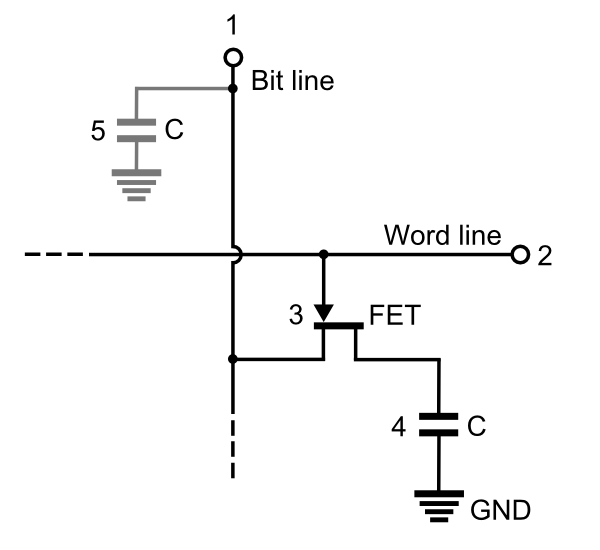
\includegraphics[scale=.20]{DRAM_memcell.png}
		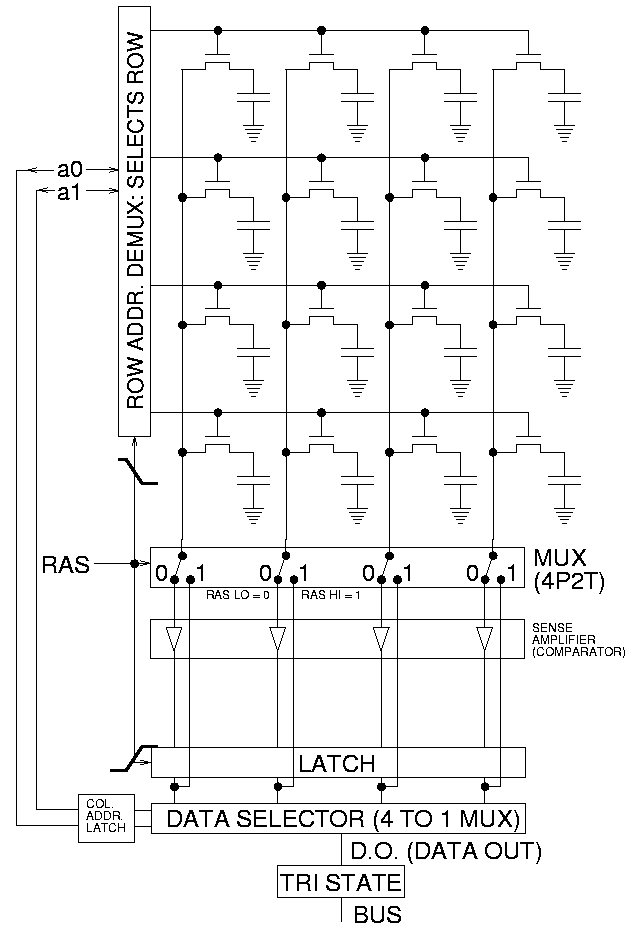
\includegraphics[scale=.10]{Square_array_memcells.png} 
		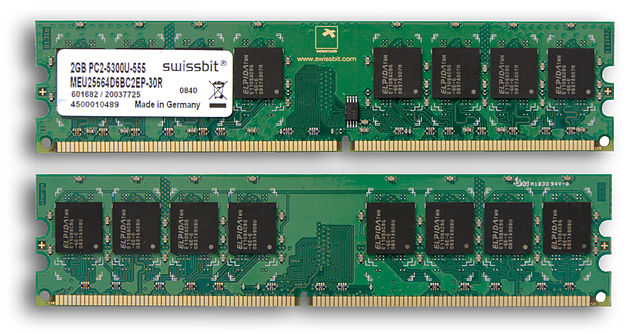
\includegraphics[scale=.50]{ramstick.jpg}
		
		\btVFill
		\href{https://en.wikipedia.org/wiki/Memory_cell_(computing)}{Wikipedia - Memory Cell} \\
		\href{https://en.wikipedia.org/wiki/Semiconductor_memory}{Wikipedia - Semiconductor Memory}
		\href{https://en.wikipedia.org/wiki/Random-access_memory}{Wikipedia - RAM}

	\end{frame}

	% Section III - Frame III
	\begin{frame}[containsverbatim] \small
	\frametitle{\sectiontitleIII}

	\underline{The Assignment Operator} \vspace{5mm} \\

	\begin{lstlisting}
	
		val_A =  53214;
	
		val_B = 0;
	
	\end{lstlisting}
	
	\begin{itemize}
		\item In C++ and many other programming languages, variables are assigned a value using the equals sign. This is called {\BL assignment}.
		\item Typically the value in the variable can be changed, or re-assigned. 
		
	\end{itemize}
	
	
	\end{frame}


% Section IV
\section{\sectiontitleIV}	
	% Section IV - Frame I
	\begin{frame}[label=sectionIV] \small
		\frametitle{\sectiontitleIV}    
		
		Question: \vspace{5mm}\\ What is the maximum number of rupees that you can hold in the original {\it Legend of Zelda} video game? 
		\vspace{25mm}
		
		Answer:

	\end{frame}

% Section V
\section{\sectiontitleV}	
	% Section V - Frame I
	\begin{frame}[label=sectionV,containsverbatim] \small
		\frametitle{\sectiontitleV}    
		
		\begin{lstlisting}

// Variables and Assigment - C++ - June 7, 2021

#include <iostream>

int main()
{
	int val = 56 ;
	
	std::cout<<"The value is: "<<val;
	
	return 0;
}
		
		\end{lstlisting}

	\end{frame}

\end{document}


%
%\begin{description}
%
%    \item [I. Components] The major building blocks of a ROS system
%
%        \begin{enumerate}
%                
%            \item \href{http://wiki.ros.org/Master}{Master Node}
%                \begin{itemize}
%                    \item {\it The ROS Master provides naming and registration services to the rest of the nodes in the ROS system.}** 
%                    \item master node runs first  {\fontfamily{qcr}\selectfont  \hspace{5mm} \$ roscore } \\
%                    \item core of the system or robot {\fontfamily{qcr}\selectfont  \hspace{5mm} \$ ROS\_MASTER\_URI=http://12345 } \\
%                    
%
%                \end{itemize}
%            
%            \item \href{http://wiki.ros.org/Nodes}{Nodes}             
%                \begin{itemize}
%                    \item {\it A node is a process that performs computation.}** 
%                    \item each 'program' or 'element' of the robot is a node\\examples:
%                        \begin{itemize} 
%                        \begin{multicols}{2}    
%                        
%                            \item sensor
%                            \item hardware driver    
%                            \item navigation 
%                            \item keyboard or joystick        
%                            
%                        \end{multicols}
%                        \end{itemize}
%                    \item start or run node individually after master\vspace{5mm}\\
%                    {\fontfamily{qcr}\selectfont  \hspace{5mm} \$ rosrun <packagename> <nodename> <options> } \vspace{1mm}\\
%                  
%                    \item all nodes are registered to the master and communicate in different ways
%                        \begin{itemize}
%                            \item  \href{http://wiki.ros.org/Topics}{topics} - publishing and subscribing
%                            \item \href{http://wiki.ros.org/Parameter%20Serverparameters}{parameter server} - static data
%                            \item \href{http://wiki.ros.org/Services}{services} - subroutine call
%                        \end{itemize}    
%                                      
%                \end{itemize}
%                
%            \item \href{http://wiki.ros.org/Packages}{Packages} 
%
%                \begin{itemize}
%                    \item {\it Software in ROS is organized in packages. A package might contain ROS nodes, a ROS-independent library, a dataset, configuration files, a third-party piece of software, or anything else that logically constitutes a useful module.}** 
%                    \item a collection of related nodes, each node belongs to a package
%                                     
%                    \item pre-built packages available with ros installation {\fontfamily{qcr}\selectfont  \hspace{5mm} -desktop-full}
%                    \item pre-built packages available for installation \\
%                    \begin{description}
%                        \item[apt] {\fontfamily{qcr}\selectfont  \hspace{1mm} \$ sudo apt-get install ros-<distribution>-<packagename> } 
%                        \item[rosdep]{\fontfamily{qcr}\selectfont  \hspace{1mm} \$ rosdep install <packagename> } \\
%                    \end{description}
%                    \item update ubuntu before installing anything \\
%                    {\fontfamily{qcr}\selectfont  \hspace{2mm} \$ sudo apt-get update } \\
%                    {\fontfamily{qcr}\selectfont  \hspace{2mm} \$ sudo apt-get check }                
%                \end{itemize}            
%
%                
%                
%    \end{enumerate}
%    ** from (ros.org)
%    \newpage
%    
%    \item [II. The Graph of the System] ROS works on a system of interconnected nodes. It is very useful to visualize this in a graph.\\
%        \begin{enumerate}   
%            
%            \item \href{http://wiki.ros.org/rqt_graph}{RQT Graph} A very useful tool. A node {\it rqt\_graph} in a package {\it rqt\_graph}. \\\\
%                    {\fontfamily{qcr}\selectfont  \hspace{5mm} \$ rosrun rqt\_graph rqt\_graph}\\
%            
%            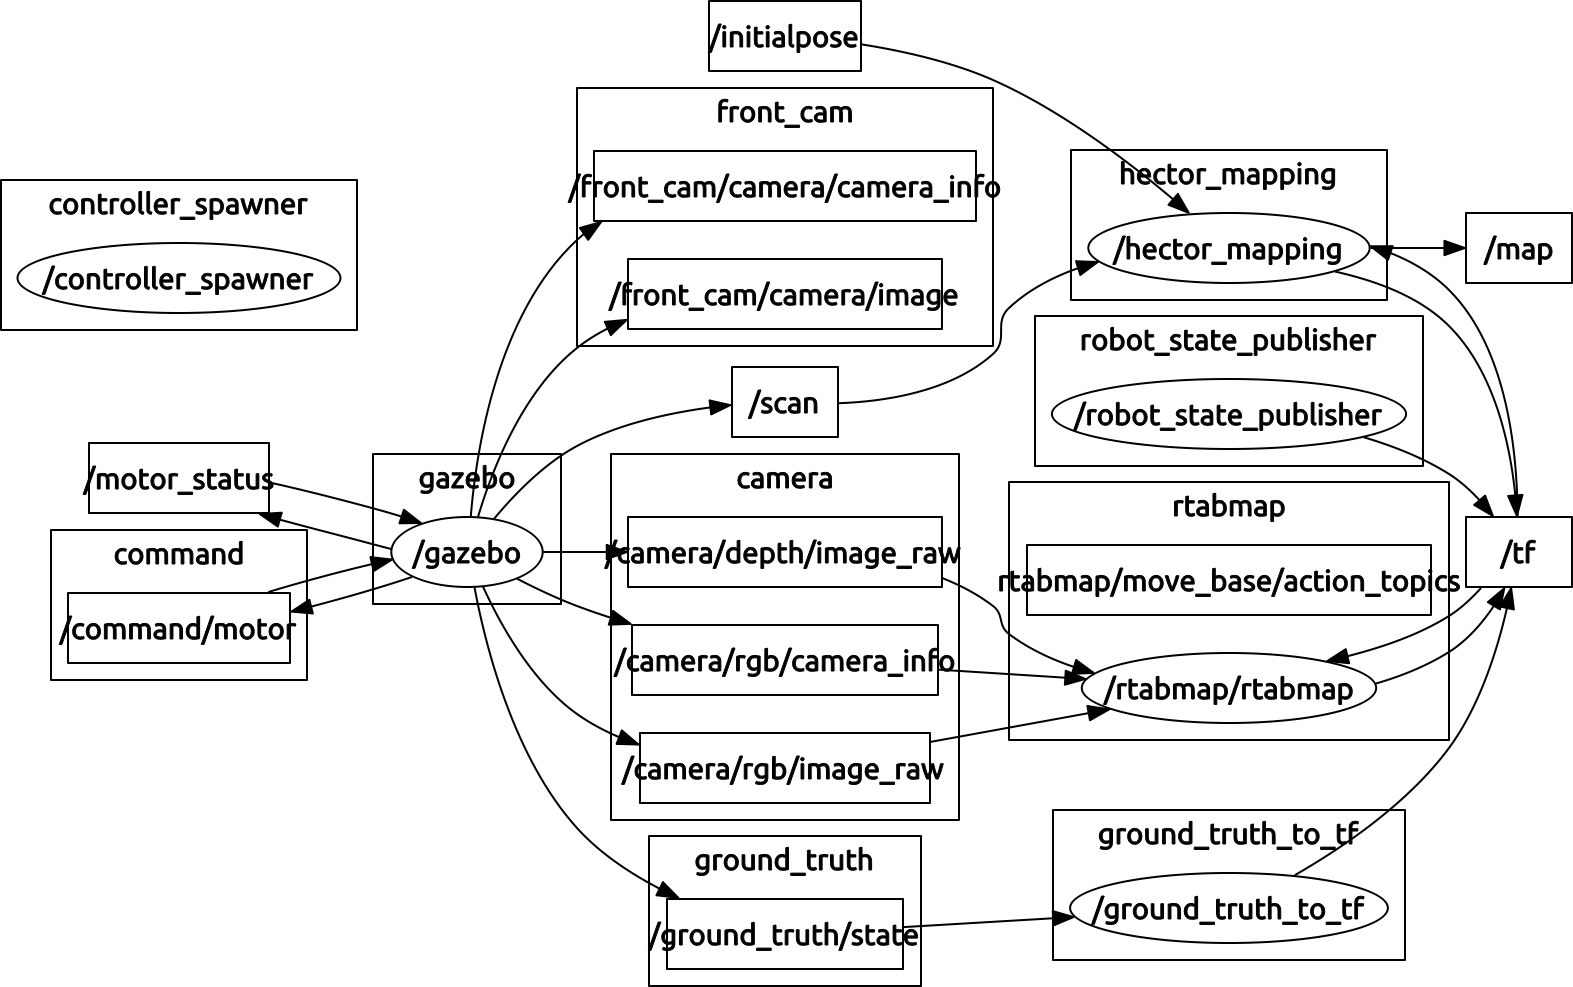
\includegraphics[scale=.4]{ros_basics_fig1.png} \\
%            
%            \item \href{http://wiki.ros.org/rqt_plot}{RQT Plot} A very useful tool. A node {\it rqt\_plot} in a package {\it rqt\_plot}. \\
%                {\fontfamily{qcr}\selectfont  \hspace{5mm} \$ rosrun rqt\_plot rqt\_plot}\\
%            
%            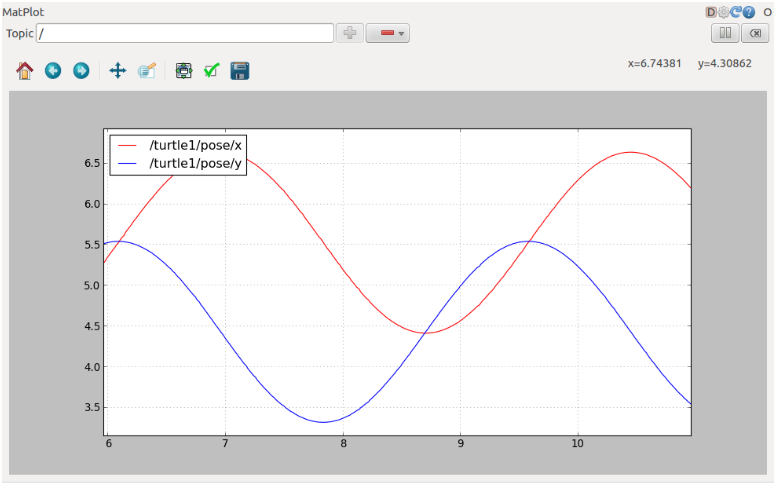
\includegraphics[scale=.5]{ros_basics_fig2.png} \\    
%          \end{enumerate}       
%
%
%\newpage
%    
%    \item [III. Topics, Publishers, and Subscribers] The nodes in a ROS system communicate.  
%        \begin{enumerate}   
%           \item \href{http://wiki.ros.org/Topics}{Topics} 
%                    \begin{itemize}
%                        \item data available to nodes in the system
%                        \item each topic has a name    
%                        \item data is stored and transferred in standard ros data types
%                        \item generally data is streaming, but does not have to be
%                    \end{itemize}    
%           \item \href{http://wiki.ros.org/ROS/Tutorials/WritingPublisherSubscriber(c++)}{Publishers}
%                    \begin{itemize}
%      
%                        \item data produced by a node can be shared with the system by publishing a topic
%                        \item a node which outputs topic data is a publisher
%                        \item a node may publish multiple topics 
%                        
%                        \end{itemize}  
%            \item \href{http://wiki.ros.org/ROS/Tutorials/WritingPublisherSubscriber(c++)}{Subscribers}
%                \begin{itemize}
%      
%                        \item a registered node can access the data in a topic by subscribing to a topic
%                        \item a node which gets topic data as input is a subscriber
%                        \item a node may subscribe to multiple topics 
%                    \end{itemize}  
%                    
%            \item \href{http://wiki.ros.org/rostopic}{rostopic}                    
%                \begin{itemize}   
%                    \item a very useful tool, a built in package 
%                    \item used differently than other packages, does not require rosrun
%                    \item a set of different tools
%                    \begin{description}   
%                        \item [list] {\fontfamily{qcr}\selectfont  \hspace{5mm} \$ rostopic list}\\
%                        \item [echo] {\fontfamily{qcr}\selectfont  \hspace{5mm} \$ rostopic echo /topicname}\\
%                        \item [type] {\fontfamily{qcr}\selectfont  \hspace{5mm} \$ rostopic pub /topicname}\\
%                    \end{description}  
%                \end{itemize}    
%                    \item  \href{http://wiki.ros.org/msg}{data types} - topics are published in standard types called messages
%                    \begin{itemize}
%                        \item {\fontfamily{qcr}\selectfont  \hspace{5mm} std\textunderscore msgs/int32 }
%                        \item {\fontfamily{qcr}\selectfont  \hspace{5mm} std\textunderscore msgs/float32 }\\
%                        
%                        \item {\fontfamily{qcr}\selectfont  \hspace{5mm} geometry\textunderscore msgs/Point }
%                        \item {\fontfamily{qcr}\selectfont  \hspace{5mm} geometry\textunderscore msgs/Pose }\\
%                        
%                        \item {\fontfamily{qcr}\selectfont  \hspace{5mm} nav\textunderscore msgs/Odometry }
%                        \item {\fontfamily{qcr}\selectfont  \hspace{5mm} nav\textunderscore msgs/Path }\\
%                    \end{itemize}
%                    
%                    \item let show an example now!
%                                      
%        \end{enumerate}     
%\newpage
%    
%%    \item [IV. Services] The nodes in a ROS system can also communicate through services. Thsi is for reply/request type operations.  
%%  \begin{enumerate} 
%%\item \href{http://wiki.ros.org/Services}{Services}
%%\end{enumerate}    
%%\newpage
%    
%
%\end{description}
%\end{document}
%
